\chapter{Algebraic Review}
\label{ch:algebra}

In this chapter we shall discuss algebraic theoretical background that grounds cryptography schemes.


\section{Basic structures}
% groups, quotient groups, cosets, rings, quotient rings, fields

\begin{definition}[Group]

A non-empty set G is called a group under the operation $*$, if it satisfies the following three axioms:

\begin{alineas}
    \item  (Closure) G is closed under $*$, i.e, for all $a,b\in G$, the result $a*b$ is also in $G$;
    \item (Associativity) $(a* b)* c = a\times (b*c)$, for all $a,b,c\in G$;
    \item (Existence of identity) There exists $e\in G$ such that $a*e=e*a=a$ for all $a\in G$;
    
    We shall denote the group as $(G,*)$. If, in addition to the above axioms, the group also satisfies the next property, it is called an \textbf{abelian group}.
    
    \item (Commutativity) For all $a,b\in G$, $a*b=b*a$.
\end{alineas}
\end{definition}

A set $R$ is called a (commutative) \textbf{Ring} if it has two operations: addition ($+$) and multiplication ($\times$) satisfying the following properties:

\begin{itemize}
    \item $R$ is an abelian group under addition
    \item (multiplicative associativity) $(a\times b)\times c = a\times (b\times c)$, for all $a,~b,~c\in R$ ;
    \item (distributivity) $a\times (b+c)=a\times b + a\times c$ for all $a,~b,~c\in R$;
    \item (multiplicative commutativity) $a\times b=b\times a$ for all $a,~b\in R$;
    \item (multiplicative inverse) There exists an element $1$, such that, $1\times a = a\times 1 = a,$ for all $a\in R$.
\end{itemize}

\section{Polynomial Rings}

\section{Cyclotomic polynomials and its properties}

In this section, we define and review some properties of cyclotomic polynomials, which will play a central role in the homomorphic cryptography setup.

\begin{definition}[Roots of unity] The $n^{th}$ roots of unity are the solution set of the equation $x^n-1=0$ in the field of complex number $\mathbb C$:
$$\sqrt[n]1=\{\zeta_n^k;k=0,1,\ldots,n-1\},$$
where\footnote{In Euler's notation $\exp{(i\theta)}=\cos\theta+i\cdot\sin\theta$} $\zeta_n=\exp{(2\pi i/n)}$
\end{definition}
In the complex plane, this roots are distributed over the unitary circumference and equally separated by an angle of $2\pi/n$. Figure \ref{fig:roots_of_unity} show the example of the $8^{th}$ roots of unity.

\begin{figure}[!htb]
    \centering
    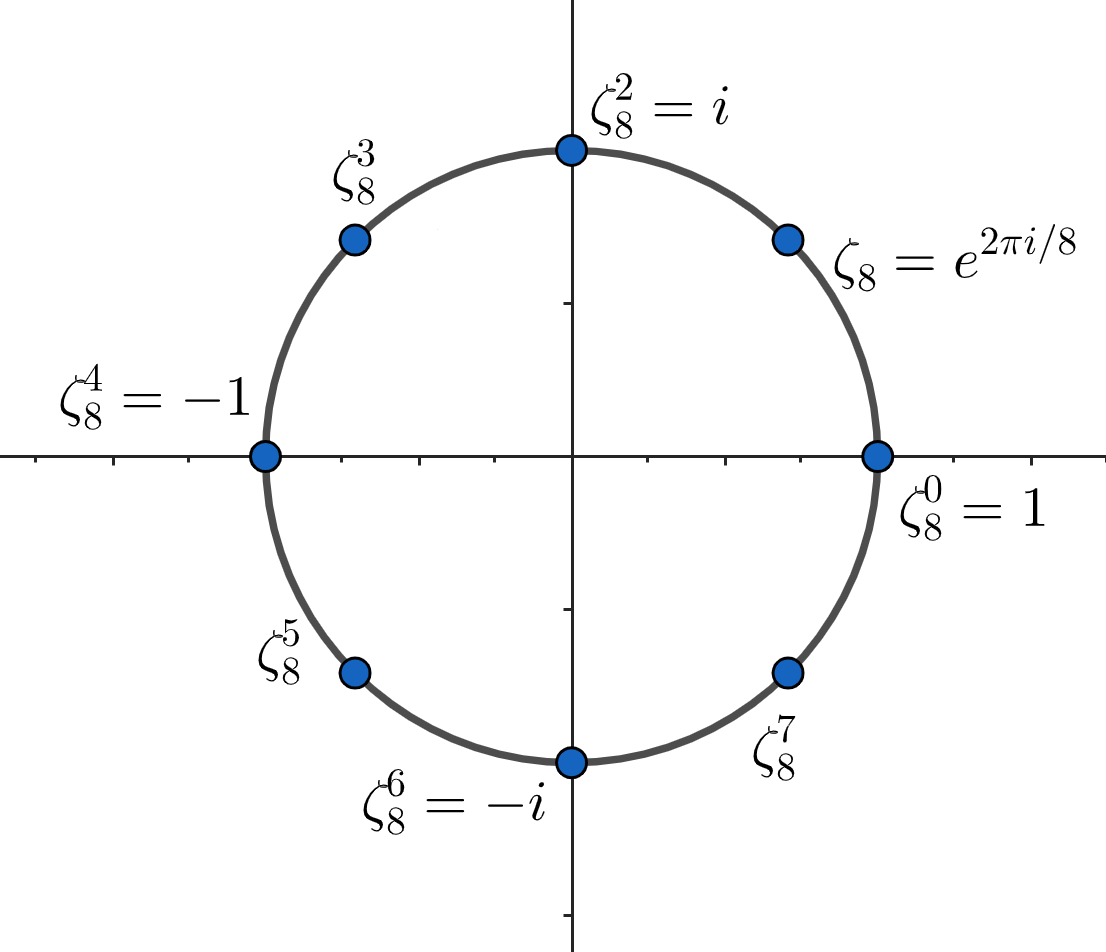
\includegraphics[scale=0.4]{files/figures/roots_of_unity.png}
    \caption{$8^{th}$ roots of unity}
    \label{fig:roots_of_unity}
\end{figure}

\begin{definition}[Primitive roots of unity]\cite{brilliant}
The $n^{th}$ primitive roots of unity are:
$$\{\zeta \in \mathbb C;\zeta^n=1\text{ and }\zeta^k\neq1,\forall ~ k<n \},$$
for positive integers $k$. They are the subset of $n^{th}$ roots of unity which are not $k^{th}$ roots of unity, for all $k<n$. They can be alternatively defined as:
$$\{\zeta_n^k;1\leq k \leq n,\gcd(k,n)=1\}$$
\end{definition}
From the Figure \ref{fig:roots_of_unity} example, the $8^{th}$ primitive roots of unity are $\zeta_8,\zeta_8^3,\zeta_8^5,\zeta_8^7$.
% Indeed, $\zeta_n^k=\exp(2k\pi i/n)$ will be equal to $1$ if, and only if the exponent is an integer multiple of $2\pi i$, which is not the case when $\gcd(k,n)=1$, since $k/n$
% tmp\cite{brilliant}

\begin{definition}[Cyclotomic polynomial] \label{def:cyclo}The \textit{$n$-th cyclotomical polynomial} is defined as:
\begin{align*}
    \Phi_n(x) = \prod_{\substack{1\leq k \leq n\\ \gcd(k,n)=1}}^{n}(x-\zeta_n^k)
\end{align*}
\end{definition}

Notice that its roots are the $n^{th}$ primitive roots of unity.

Using the definition, we can derive some cyclotomical polynomials, for example $\Phi_1(x)=x-1$ trivially, and $\Phi_2(x)=x+1$, since from the $2^{nd}$ roots of unity $-1$ and $+1$, only $-1$ are primitive ones.

The $3^{rd}$ primitive roots of are $\zeta_3^1$ and $\zeta_3^2=\overline{\zeta_3^1}$, then:
\begin{align}
    \Phi_3(x)&=(x-\zeta_3^1)(x-\zeta_3^2)\nonumber\\
    &=x^2-x(\zeta_3^1+\zeta_3^2)+\zeta_3^1\zeta_3^2\nonumber\\
    &=x^2-x(\zeta_3^1+\overline{\zeta_3^1})+e^{2\pi i(1+2)/3}\label{eq:zeta3}\nonumber\\
    &=x^2-x(2\cdot\cos(2\pi/3))+e^{2\pi i}\\
    &=x^2+x\left(2\cdot \frac12\right)+1\nonumber\\
    &=x^2+x+1\nonumber
\end{align}

The equality (1) holds due to the sum of complex conjugates being equal to two times the real part since we cancel out the imaginary terms.

\begin{theorem} \label{teoremaco}For all positive integers $n$ we have:
$$\displaystyle x^n-1=\prod_{d|n}\Phi_d(x)$$
\end{theorem}

The above theorem provides a analytical formula to recursively generate the cyclotomic polynomials:
$$\displaystyle\Phi_n(x)=\dfrac{x^n-1}{\displaystyle\prod_{\substack{d|n\\d\neq n}}\Phi_d(x)}$$

We can use it to derive simpler, and non-recursive expressions for particular interesting cases:

\begin{corollary}[Prime Cyclotomical Polynomial]
If $p$ is a prime number, then:
$$\Phi_p(x)=x^{p-1}+x^{p-2}+\ldots+x+1$$
\end{corollary}

\begin{proof}
By the previous theorem, and the fact that the only $d<p$ satisfying $d|n$ is $d=1$:

$$\Phi_p(x)=\dfrac{x^p-1}{\displaystyle\prod_{\substack{d|p\\d\neq p}}\Phi_d(x)}=\dfrac{x^p-1}{\Phi_1(x)}=\dfrac{x^p-1}{x-1}$$

The polynomial division algorithm concludes that such a division actually results in what is claimed in the corollary.

An easy way to assert it, is by multiplying the divisor $x-1$ by $\displaystyle\sum_{i=0}^{p-1}x^i$ and checking if it is equal to $x^p-1$:
\begin{align*}
    (x-1)\left(\sum_{i=0}^{p-1}x^i\right)&=\sum_{i=0}^{p-1}x^{i+1}-\sum_{i=0}^{p-1}x^i\\
    &=\sum_{i=0}^{p-1}x^{i+1}-x^{i}\\
    &=x^{(p-1)+1}-x^{0}\\
    &=x^{p}-1
\end{align*}
\end{proof}
The following formula will be crucial to instantiate plaintext and cyphertext spaces in the encryption schemes.
\begin{corollary}[Power of Two Cyclotomic Polynomial]
If $M=2^n$, for a given positive integer $n$, then:
$$\Phi_M(x)=x^{M/2}+1$$
\end{corollary}
\begin{proof}
We'll proceed by strong induction in $n$ \cite{herstein1996abstract},  proving an equivalent statement\footnote{One can easily verify that $\dfrac{x^{M}-1}{x^{M/2}-1} = x^{M/2}+1$ using the polynomial division algorithm for example, or multiplying the divisor with the quotient}: 
\begin{equation}
\label{eq:phim}
    \Phi_{M_n}(x) = \dfrac{x^{M_n}-1}{x^{M_n/2}-1}
\end{equation}
We're denoting $2^n$ by $M_n$ to have a cleaner notation of nested exponents; hence $M_n/2=M_{n-1}$.

(Base case) For $n=1$, $\Phi_{M_1}(x)=\Phi(2)=x+1$, as we derived before. This is the LHS of \ref{eq:phim}. The RHS is $\frac{x^2-1}{x-1}=\frac{(x+1)(x-1)}{x-1}=x+1$, so the formula is valid in this case.

(Inductive Hypothesis) Assume that \ref{eq:phim} hold for $M_k$ for all $k<n$ positive integers.

(Inductive Step) Let's deduce that it also holds for $M_n$: By Theorem  \ref{teoremaco}, we have:
\begin{align*}
    \Phi_{M_n}(x) &= \dfrac{x^{M_n}-1}{\displaystyle\prod_{\substack{d|M_n\\d\neq M_n}}\Phi_d(x)}
\end{align*}
Notice that $\{d\in\mathbb{Z}^+;d|M_n\} = \{M_0,M_1,\ldots,M_{n-1}\}$, i.e., the divisors of $M_n$ are the powers of two with exponent less than $n$. Then our expression becomes:
$$\Phi_n(x) = \dfrac{x^{M_n}-1}{\Phi_{M_0}\Phi_{M_1}\ldots\Phi_{M_{n-1}}}$$
Using $\Phi_{M_0}(x)=x-1$ and the inductive hypothesis we can rewrite the denominator as:
\begin{align*}\Phi_{M_0}\Phi_{M_1}\ldots\Phi_{M_{n-1}}&=(x-1)\cdot \dfrac{x^{M_1}-1}{x^{M_0}-1}\cdot\dfrac{x^{M_2}-1}{x^{M_{1}}-1}\ldots\cdot\dfrac{x^{M_{n-1}}-1}{x^{M_{n-2}}-1}\\&=x^{M_{n-1}}-1,\end{align*}
since that's the only term left after cancelling out left numerators with right denominators. We then conclude:
\begin{align*}
    \Phi_{M_n}(x) &= \dfrac{x^{M_n}-1}{x^{M_{n-1}}-1}=x^{M_n/2}+1
\end{align*}
\end{proof}

Another interesting property of cyclotomic polynomials which is quite impressive, is the following theorem:
\begin{theorem}
``For any positive integer $n$ we have $\Phi_n(x)\in\Z[x]$, That is, $\Phi_n(x)$ is a polynomial
with integer coefficients.''\cite{sun2013cyclotomic}
\end{theorem}
We defined these polynomials as products of a bunch of complex numbers, but the coefficients end up in the integers! Such a beautiful property will allow us to determine later quotient rings like $\Z[x]/(\Phi_n(x))$ to our encryption context.

\section{Lattices}

This section introduces lattices and hard lattice problems that will base the security of fully homomorphic schemes.
\begin{definition}[Lattice]
Let $b_1,\ldots,b_k\in\mathbb{R}^n$ be linearly independent vectors, then
$$\mathcal{L}=\Big\{\sum_{i=1}^ky_ib_i\left|\right.y_i\in\mathbb{Z}\Big\}$$
is a ($n$-dimensional) \textbf{lattice} and $(b_1,\ldots,b_k)$ its \textbf{basis}. If we create a $n\times k$ matrix $\mathbf B$, where the $i$-th column is $b_i$, then we can write
$$\mathcal{L}(\mathbf B)=\{\mathbf B y| ~y\in \mathbb{Z}^k\}\subset \operatorname{span}(B)$$
\end{definition}
Figure \ref{fig:lattices} shows two geometrical examples in $\R^2$, the first one using canonical basis $(e_1,e_2)$, and the second suing $B=(b_1,b_2)$, with $b_1=e_1$ and $b_2=\frac{1}{\sqrt2}(2,1)$
\begin{figure}[!htb]
\centering
\begin{subfigure}{.5\textwidth}
  \centering
  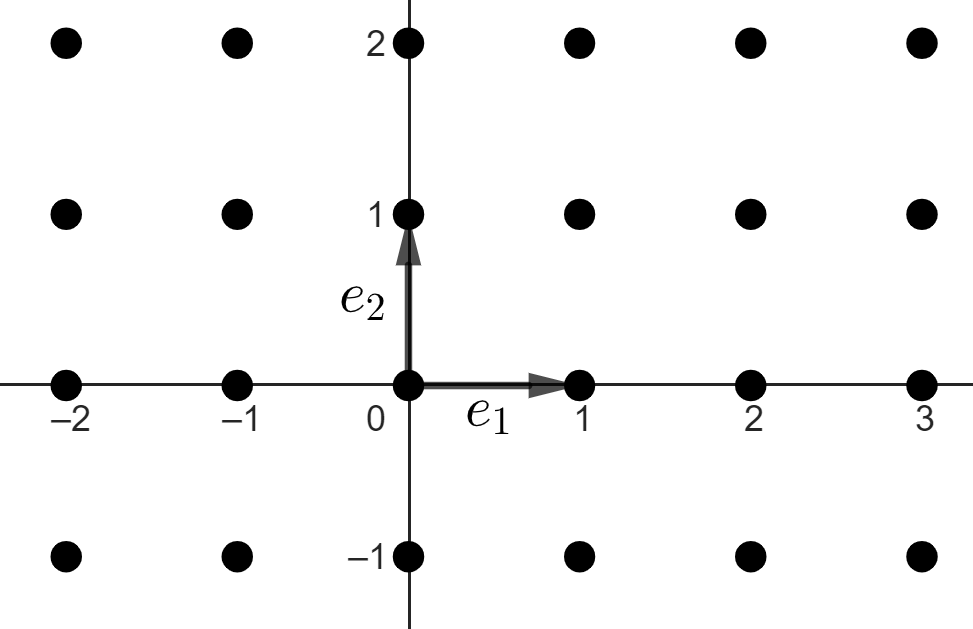
\includegraphics[scale=0.25]{files/figures/lattice_canonical.png}
  \caption{Canonical basis}
  \label{fig:canonical_lattice}
\end{subfigure}%
\begin{subfigure}{.5\textwidth}
  \centering
  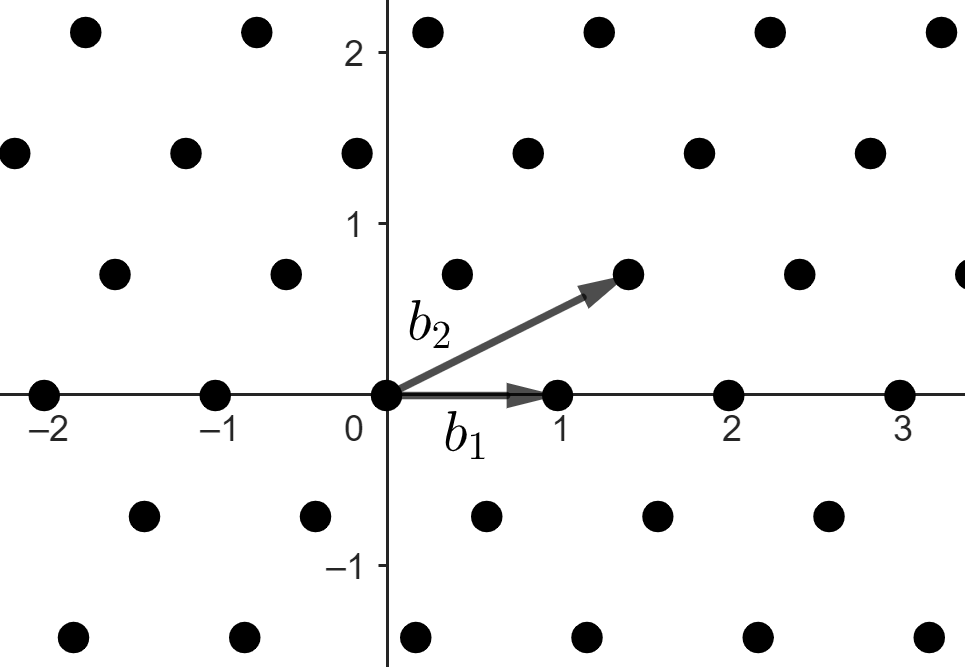
\includegraphics[scale=0.25]{files/figures/lattice2.png}
  \caption{Basis $B=(b_1,b_2)$}
  \label{fig:sub2}
\end{subfigure}
\caption{Lattices examples}
\label{fig:lattices}
\end{figure}

\begin{definition}[Ideal lattice]
An \textbf{ideal lattice} $\mathcal L$ is a lattice that is closed under addition and multiplication: For $v_1,v_2\in \mathcal{L}$, we have $v_1+v_2\in \mathcal{L}$ and $v_1\cdot v_2\in\mathcal L$, with the operations inherited by $\R^n$
\end{definition} 

\begin{definition}[Successive minima]
The $i^{th}$ successive minima of an $n$-dimensional lattice $\mathcal L$, denoted by $\lambda_i(\mathcal L)$ is the smallest $r$ such that origin-centered ball with radius $r$ contains $i$ linearly independent (LI) lattice vectors.
\end{definition}

In Figure \ref{fig:canonical_lattice} example $\lambda_1(\mathcal L)=\lambda_2(\mathcal L)=1$, since the unity ball contains the two LI canonical vectors. But in Figure \ref{fig:sub2}, it's not so obvious, but $\lambda_1(\mathcal L)=||b_3||_2\approx 0.82$, where $b_3=b_2-b_1$ and $\lambda_2(\mathcal L) = ||b_4||_2\approx0.92$, with $b_4=b_3-b_1$. In Figure \ref{fig:successive_minimas} we can visually verify that $b_3$ and $b_4$ are indeed LI.

\begin{figure}[!htb]
\centering
\begin{subfigure}{.5\textwidth}
  \centering
  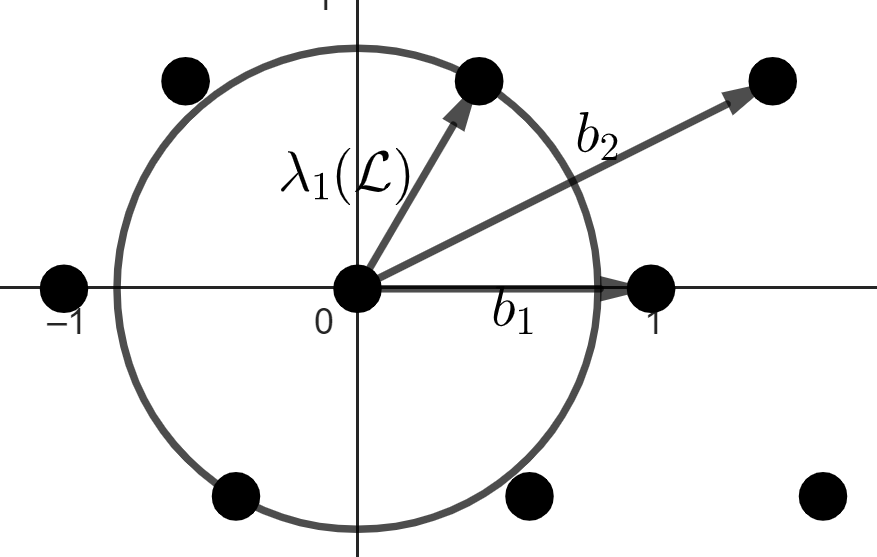
\includegraphics[scale=0.25]{files/figures/lambda1.png}
  \caption{$1^{st}$ successive minima}
  \label{fig:lambda1}
\end{subfigure}%
\begin{subfigure}{.5\textwidth}
  \centering
  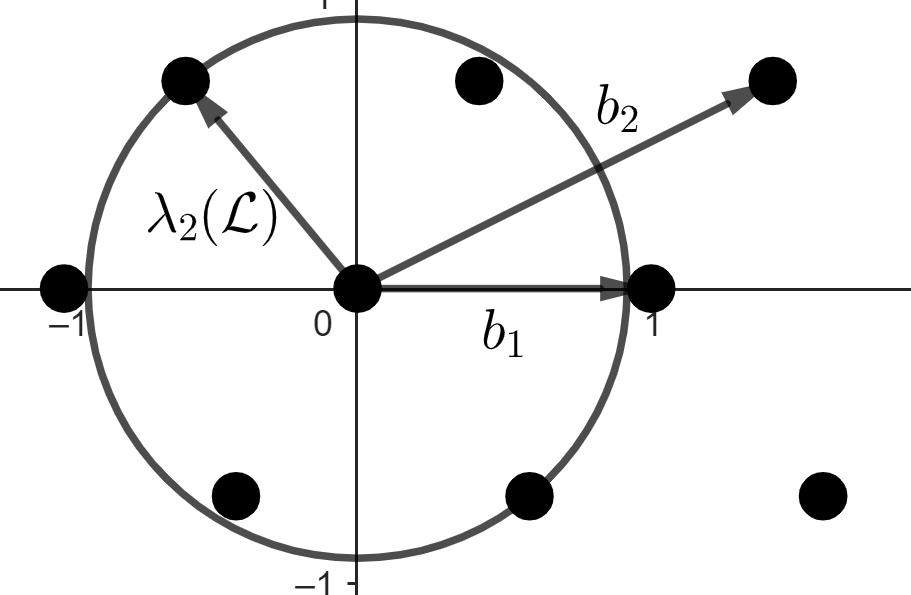
\includegraphics[scale=0.23]{files/figures/lambda2.png}
  \caption{$2^{nd}$ successive minima}
  \label{fig:lambda2}
\end{subfigure}
\caption{Successive Minimas}
\label{fig:successive_minimas}
\end{figure}

\subsection{Lattice Problems}
Now we can define two famous lattice problems, all of them considered NP-hard \cite{hardnes}. ``The approximation factor $\gamma$ is usually taken as a function of lattice dimension $\gamma(n)$.'' \cite{ppt_dm}

\begin{definition}[Shortest Vector Problem - SVP]\label{def:svp} Given a lattice $\mathcal L$ and a norm $||.||$, find a non-zero $v\in\mathcal L$ such that $||v||\leq\gamma \lambda_1(\mathcal L)$, i.e., the non-zero lattice vector closest to the origin. 
\end{definition}

In the above example of $\mathcal L (b_1,b_2)$ the shortest vector is $b_3$, for $\gamma=1$.

\begin{definition}[Shortest Independent Vector Problem - SIVP] Given a lattice $\mathcal L$ of dimension $n$ and a norm $||.||$, find $n$ linearly independent vectors $v_1,v_2,\ldots,v_n$ such that $\displaystyle\max_{i}{||v_i||}\leq\gamma\lambda_n(\mathcal L)$.
\end{definition}

For $\mathcal L (b_1,b_2)$, the solution for the $\text{SIVP}_\gamma$ with $\gamma=1$ is $\{b_3,b_4\}$.

These problems establish the so-called \textit{lattice-based cryptography}, which are cryptosystems that have their security based on solving the above problems of variants. All The fully homomorphic encryption schemes we shall dive deeper into in the next chapter are lattice-based.

\subsection{Ring Learning with Errors}
Now that we have computationally complex challenges, the next step is, based on these results, constructing a concrete secure cryptography scheme. The following two problems are a step in this direction.

\begin{definition}[Learning with Errors - LWE] Given an integer $n$, a prime integer $q$ such that\footnote{$\poly(n)$ denotes a polynomial function of $n$.} $2\leq q\leq \poly(n)$ and a distribution $\chi$ over $\Z_q$. Fix $\bds\in \Z_q^n$, the Search $\operatorname{LWE}_{n,q,\chi}$ problem is to recover $\boldsymbol s$, given observations $(\bda_i,b_i)$, where\footnote{Notation $x\xlongleftarrow[]{\chi}S$, means $x$ were drawn from distribution $\chi$ over the set $S$, and $\mathcal{U}$ is the uniform distribution}:
\begin{align*}
    \bda_i&\xlongleftarrow[]{\mathcal U}\Z_q^n\\
    b_i &= \langle \bda_i,\bds\rangle + e_i\\
    e_i&\xlongleftarrow[]{\chi}\Z_q
\end{align*}
The Decision $\operatorname{LWE}_{n,q,\chi}$ is the problem of distinguishing between the distribution of $(\bda_i,b_i)$ gotten from the above procedure and the uniform distribution over $\Z_q^{n+1}$.
\end{definition}
Under reasonable assumptions on $\chi$, if an algorithm efficiently solves the above (decision) problem, GapSVP and SIVP can also be solved efficiently \cite{regev09}. 

LWE provides a nice setup for private key encryption since one can expose $(\bda_i,b_i)$ while the hardness of lattice-based problems guarantees security of $\bds$. Further, we shall name $(\bda_i,b_i)$ as the public key and $\bds$ as the private key. One can still proved that Seach-LWE can be reduced to Decision-LWE \cite{lyubashevsky10} which completes the cycle.

In our main FHE construction, the scheme is actually bases on a variant of LWE:

\begin{definition}
[Ring Learning with Errors - RLWE] Set integers $n,q$, with $n$ being a power of two, and $2\leq q \leq \poly(n)$. Let $f(x)=x^n+1$ (the $2n$-th cyclotomic polynomial), define $R=\Z[x]/\langle f(x)\rangle$, a distribution $\chi$ over $R$ and $R_q=R/\langle q\rangle =\Z_q/\langle f(x)\rangle$ which can be represented by polynomials with integer coefficients wrapped by $q$ and with degree up to $n-1$.

Let $s=s(x)\in R_q$ be an element chosen uniformly from the ring. The Search $\operatorname{RLWE}_{n,q,\chi}$ problem is to recover $s$ given a set of pairs $(a_i,b_i)\in R_q^2$, with
\begin{align*}
    a_i&\xlongleftarrow[]{\mathcal U}R_q\\
    b_i &= a_i\cdot s + e_i\\
    e_i&\xlongleftarrow[]{\chi}R
\end{align*}
Analogously with LWE, we define Decision $\operatorname{RLWE}_{n,q,\chi}$ as the problem of distinguishing the distribution of the above pairs from a uniform distribution over $R_q^2$. 
\end{definition}

An observation in both LWE and RLWE is that, in practice, the distribution $\chi$ of $e_i$ must yield small enough errors compared to $q$. That's why we omit $\bmod q$ after the equation of $b_i$'s. Such a thing would guarantee that $b_i$ is an element of $\Z_q$ or $R_q$.

The Search RLWE can also be reduced to Decision RLWE. Moreover, under some assumptions over the parameters $n,q,\chi$, which we won't state here, an efficient algorithm for Decision $\operatorname{RLWE}_{n,q,\chi}$ implies an efficient algorithm for solving SVP \cite{lyubashevsky10}.
% $\boldsymbol a$ is taken uniformly from $\Z_q^n$ and $b=\langle \boldsymbol s,\boldsymbol$



\chapter{Fully Homomorphic Encryption}
This chapter gives an over view of the FHE research. Section \ref{sec:privhom} get back in 1978 and revises the original proposal of the existence of FHE schemes. Section \ref{sec:gentry} explore Gentry's solution through his PhD thesis \cite{gentry2009fully} proving such existence. Section \ref{sec:ckks} presents the so called CKKS scheme \cite{ckks17}, a practical and modern scheme that allows approximate encryption of complex (so, also real) number, very suitable for machine learning applications. 

\section{Privacy Homomorphisms}
\label{sec:privhom}
Assume we can represent the unencrypted data by an algebraic structure $\mathcal P= (S;f_1,\ldots,f_k)$, i.e., a set $S$ ported with the operations $f_1,\ldots,f_k$. We will further call this structure the plaintext space.

An alternative algebraic structure, the cyphertext space $\Cypher=(S',f'_1,\ldots,f'_k)$, is constructed to represent the encrypted data. To build a \textit{privacy homomorphism} \cite{Rivest1978},  one needs a decryption function $\phi:S'\to S$ and its inverse $\phi^{-1}:S\to S'$ satisfying the homomorphic property from $\Cypher$ do $\Plain$:
\begin{align}
    \label{privhom}
    f'_i(a,b,\ldots)&=c\Rightarrow\nonumber\\ f_i(\phi(a),\phi(b),\ldots)&=\phi(c),\text{ for } i=1,\ldots,k\\
    \text{with }a,b,&\ldots\in S'\nonumber
\end{align}
This means that for all available operations $f'_i$, its evaluation on encrypted elements must result in a value that, after decryption, corresponds to the same computation on the unencrypted domain.

An example of privacy homomorphism is the RSA cryptosystem \cite{rsa}, which uses $\Plain = (\Z_p;\times_p)$, the integers modulo $p$ with $p$ prime, and the multiplication modulo $p$. Setting $N=pq$, where $q$ is a large prime and choosing $e$ coprime with $(p-1)(q-1)$,  the cyphertext space as $(\Z_N;\times_N)$ and is connected with $\Plain$ through the encryption function:
\begin{align*}
    \phi^{-1}&:\Z_p\to\Z_N\\
    \phi^{-1}(x)&=x^e(\bmod N)
\end{align*}
Taking $x,y\in\Z_p$ and its encrypted versions $x'=\phi^{-1}(x),~y'=\phi^{-1}(y)$, we have:
\begin{align*}
    x'\times_N y'&= (x^e)(y^e)(\bmod N)\\
    &=(xy)^e(\bmod N),
\end{align*}
which is an encryption of $xy$. Then the multiplication satisfies property \ref{privhom}, showing that such a system is indeed a privacy homomorphism.

\subsection{Requirements and Limitations}
The following properties for $\Cypher,\phi$ and $\phi^{-1}$ are required by the authors:
\begin{alineas}
    \item for a given element $s\in S$, its encrypted version $\phi^{-1}(s)$ should not require much more storage space;
    \item $\phi$ and $\phi^{-1}$ should be easy to compute;
    \item the operations $f_i'$ should be efficiently computable in $\Cypher$;
    \item $\phi$ should not be vulnerable to the chosen plaintext attack;
    \item The operations of $\Cypher$ should not be sufficient to yield an efficient computation of $\phi$.
\end{alineas}

The last requirement forces a critical restriction on such morphisms: a comparison operator ``$\leq$'' can't be available in the cyphertext space, otherwise, no secure privacy homomorphism exists.

Take for example $\Plain = (\N;+,\leq)$ and $\Cypher = (W;+',\leq')$ for some $W$. A malicious party who has $\phi^{-1}(n)$, and wants to discover what $n\in\N$ generated such cyphertext can apply the following binary search strategy:
\begin{alineas}
\item compute $1'=\phi^{-1}(1)$;
\item compute $2'=1'+'1'$, then $4'=2'+'2'$;
\item continue until finding $k$, such that $\phi^{-1}(n)\leq'(2^k)'=\phi^{-1}(2^k)$
\item knowing that $n\in[2^{k-1},2^{k}]$, compute an encryption of the interval midpoint $\phi^{-1}(m)=\phi^{-1}(2^{k-1}-2^{k-2})$;
\item homomorphically compare $\phi^{-1}(n)\leq'\phi^{-1}(2^{k-1})+'\phi^{-1}(m)$;
\item repeat the last two steps properly redefining the interval until getting $n$ exactly.
\end{alineas}
This is an efficient $O(\log n)$ algorithm to compute the decryption function $\phi$, using the operations in $\Cypher$ and the ability to generate encryptions of arbitrary constants (such as $1$ and $m$ in the above example).

The article finishes with the authors pondering if such an approach with all required security restrictions could be worthwhile in practice and what algebraic structures $\Plain$ would provide useful privacy homomorphisms.
% \section{First Generation Fully Homomorphic schemes}
% \begin{alineas}
% \item somewhat/fully homomorphic
% \item bootstrapping
% \item integer scheme
% \item caveats and implementation paper
% \end{alineas}

\section{Gentry's contribution}
\label{sec:gentry}

% \section{Gentry's work}


% \subsection{BFV and BGV schemes (integers)}

% \begin{alineas}
% \item describe BFV primitives (codec/ring)
% \item encrypt/decrypt
% \item relinelization
% \item BGV differences
% \end{alineas}

\section{Approximate Numbers Homomorphic Encryption}
\label{sec:ckks}

- brief description about fixed point arithmetic? no 
- the complex map 
- give a broad overview and then in subsection describe codec and bootstrapping

\subsubsection{Encoding and Decoding}


\subsection{Approximate Bootstrapping}

\chapter{Private Logistic Regression}
\section{Statistical Review}
\section{Homomorphic Training}
\section{Data Applications}


\label{ch:algebra}

